\chapter{Materiais}
\begin{itemize} %% TODO: colocar as rodas: http://www.hobbyking.com/hobbyking/store/__2176__598__Hardware_Accessories-Wheels_0_40mm.html
 \item 5 sensores ultrassônicos de distância HC-SR04
 \item 2 motores \textit{brushless outrunner} Turnigy D2836/9 950KV
 \item 2 ESCs Hobby King com UBEC de 5.5V/4A: um de 35A e outro de 40A 
 \item 2 módulos de rádio frequência baseados no \textit{transceiver} Nordic nRF24L01+ 
 \item 1 bateria LiPo 30C de 2800 mAh
 \item 2 Arduino Pro Mini
 \item 1 Conversor/Adaptador USB-Serial PL2303
 \item 1 Carregador balanceador de bateria IMAX B6-AC
\end{itemize}

\section{Motor \textit{Brushless}}
São motores síncronos\footnote{Motores Síncronos: o campo magnético girante do rotor e do estator têm a mesma frequência.} de corrente contínua cuja 
comutação é feita eletronicamente, e não mecanicamente por meio de escovas como nos motores CC comuns, por isso denominados \textit{brushless}.
Possui aplicações nas indústrias de automóveis, aeroespacial, médica, de equipamentos de automação industrial e instrumentação .
Os motores BLDC apresentam algumas vantagens em relação aos de corrente contínua com escovas e de indução no que concerne a: resposta 
dinâmica, ruídos 
de operação, durabilidade (i.e. vida útil), assim como razão do torque pelas dimensões do motor \cite{motor_2}. 

% TODO tava uma merda, reler pois alterei um pouco
O rotor consiste de um imã permanente, já os pólos do estator são formados por enrolamentos, que precisam ser energizados na sequência correta 
para que um campo magnético girante seja criado.
Nas máquinas CC isto é feito mecanicamente através das escovas mas, no caso do BLDC, é preciso que a posição do rotor em relação ao estator seja 
conhecida para que seja possível fazer o acionamento correta das bobinas.
Existem dois meios de se obter esta informação: através de sensores de efeito hall, método empregado neste trabalho, ou processamento da força contra 
eletromotriz das bobinas do estator.

Sensores de efeito Hall são transdutores analógicos que relacionam a intensidade do campo magnético externo transversalmente disposto a ele em termos 
de tensão elétrica. Quando associado a um circuito comparador \textit{schmitt trigger}, comportam-se como um sensor digital que aponta quando a 
intensidade do campo magnético atinge um valor de limiar pré-determinado. Ao dispor sensores deste tipo ao longo do estator, torna-se possível uma 
estimativa da posição do rotor ao ser feito um estudo comparativo da resposta de cada sensor, cruzando esta informação com a posição que 
cada um destes se encontra em relação ao estator \cite{motor_1}.

Há a possibilidade de fazer a comutação sem empregar qualquer tipo de sensor, logo, trata-se de um método mais barato. 
Nesse caso, a estimativa da posição do rotor se dá através do processamento das forças contra-eletromotriz de cada um dos enrolamentos do estator.
No entanto, algumas limitações surgem: o motor deve operar acima de uma dada rotação, caso contrário o método não funciona; mudanças bruscas de carga 
não podem ocorrer; há discontinuidades na resposta do motor quando operando em velocidades acima da taxa de comutação ideal \cite{motor_1}.

\section{ESC}
Controlador responsável por processar as informações oriundas dos sensores de efeito Hall do motor BLDC e providenciar o acionamento correto 
dos enrolamentos do estator para que a velocidade angular se dê de acordo com o sinal de controle que é enviado a este dispositivo.
No caso dos ESCs utilizados no presente trabalho, este sinal de controle é feito utilizando-se modulação por largura de pulso, i.e. PWM. 
A frequência de operação varia de acordo com o modelo do controlador e para o caso deste projeto é de 400Hz.
%% TODO: \cite{carlson}
%% TODO: fazer uma descrição mais rica de como funciona este dispositivo.
%% TODO: citar que toda a programação do ESC é feita via pwm.
\section{Sensor Ultrassônico}

\subsection{Princípio de Funcionamento}
Utiliza o método \textit{time of flight}, que consiste na medição do intervalo de tempo, igualmente denominado \textit{time of flight}, que uma onda 
ou partícula leva para percorrer uma determinada distância em um dado meio. 
Pode ser utilizado para medir: distância, velocidade \cite{TOF_velocity}e propriedades do meio de propagação ou da partícula propagante
\cite{TOF_medium1,TOF_medium2}.

Para medidores de proximidade, como é o caso de sonares e lasers, um transdutor emissor faz a conversão do sinal elétrico, denominado 
\textit{trigger}, em um pulso de ondas (acústicas para o caso do sonar e eletromagnéticas para o laser), dando início à medição de tempo.
Quando esta onda propagante encontra um objeto que a reflita de volta ao sensor e a intensidade deste sinal recebido, denominado \textit{echo}, está 
acima de um determinado valor de limiar, o transdutor receptor envia um sinal elétrico que interrompe a contagem de tempo, obtendo-se 
assim a medida do \textit{time of flight}, $\tau$.
Com isso, supondo que a velocidade de propagação, $\nu$, desta onda no meio seja conhecida. De acordo com \citeonline{siegwart}, pode-se 
calcular a distância, $\Delta$, entre o sensor e o objeto que reflete o pulso de ondas pela Eq.\ref{TOF_eq}:
\begin{equation}
 \label{TOF_eq}
 \Delta = \frac{\nu \times \tau }{2}
\end{equation}

Quanto ao sensor ultrassônico especificamente, temos que as ondas sonoras utilizadas estão usualmente situadas entre 40kHz e 180kHz, sendo 
emitidas no formato de pacotes compostos por uma série de pulsos; no caso do sonar utilizado neste trabalho, 8 pulsos de 40kHz. 
Por se tratarem de ondas mecânicas, é importante que a tensão de limiar, do inglês \textit{threshold}, comporte-se ao longo do ciclo de 
leitura da seguinte forma \cite{siegwart}: 
durante o período denominado \textit{blanking time} \cite{siegwart}  ou \textit{dead time} \cite{murphy}, o qual engloba o intervalo de 
emissão das ondas sonoras até o momento em que o diafragma para de oscilar (o que pode constituir alguns milisegundos após a cessação do sinal de 
\textit{trigger}), a tensão de limiar é muito alta no intuito de eliminar leituras inválidas decorrentes de interferência entre emissor e receptor; em 
seguida, a tensão de \textit{threshold} se reduz a um valor que permita a detecção de obstáculos e vai sendo continuamente decrementada com o passar 
do tempo. 
Isso se dá pelo fato de que a intensidade do sinal acústico, i.e. potência por ângulo sólido, sofre atenuações atmosféricas que variam com a 
distância percorrida, conforme a equação \ref{Atm_Attenuation} \cite{everett}, que leva em consideração somente efeitos da divergência esférica e 
absorção molecular.
\begin{equation}
 \label{Atm_Attenuation}
 I = \frac{ I_0 e^{-2 \alpha R} }{4 \pi R^2}
\end{equation}
Em que: $\alpha$ é o coeficiente de atenuação do meio, associado às absorções moleculares, o qual varia em função da frequência da onda emitida 
assim como de propriedades do meio, e.g. umidade e poeira contida no ar.
Para ondas de 40kHz: $\unitfrac[0,197]{dB}{m} < \alpha <  \unitfrac[0,295]{dB}{m}$. % TODO posso deixar essa desigualdade aqui???

\subsection{Limitações}

\subsubsection{Variação na velocidade de propagação da onda acústica}
Como citado anteriormente, a medição da distância pressupõe que a velocidade de propagação da onda no meio é conhecida. 
No entanto, mudanças na temperatura e umidade do fluido em que a onda se propaga podem causar erros de medida não desprezíveis \cite{everett}.

\subsubsection{Direcionalidade}
O emissor da radiação acústica ultrassônica apresenta um padrão de radiação \cite{balanis,pozar} composto por lobos laterais \cite{balanis,pozar} que 
não são levados em conta, pois a maioria dos sistemas supõem toda radiação recebida como oriunda do lobo central \cite{balanis,pozar}, usualmente 
modelado como um cone de aproximadamente $30^o$ que varre até 5 metros \cite{murphy}. De acordo com \citeonline{HC-SR04}, para o dispositivo 
utilizado nesse trabalho o ângulo de abertura do feixe é de $15^o$ e o alcance, 4 metros.

Além deste problema, o próprio fato de que a direcionalidade do sensor é baixa, i.e. o lobo central é largo, implica numa 
imprecisão na medida obtida, pois não é possível associar a distância lida a um lugar específico, mas sim a uma região no espaço coberta pelo lobo 
central \cite{siegwart}.

\subsubsection{Resposta no Ambiente Alvo}
Por ser um sensor refletivo, a performance do sonar é significativamente afetada pelas características do alvo \cite{everett}.
Um dos problemas decorrentes desse fato é que determinados objetos apresentam elevada taxa de absorção ou, ao contrário, são atravessados pela 
radiação, resultando, em ambos os casos, em pouca ou nenhuma energia retornando ao sensor. Dessa forma, estes objetos são invisíveis para o dado 
método de medição; materiais como espuma, pele e roupas podem absorver as ondas acústicas \cite{siegwart} enquanto objetos com áreas superficiais 
pequenas, e.g. mesas e cadeiras, podem não ser detectados \cite{murphy}. Vale ressaltar que as propriedades de reflexão, absorção e transmissão 
são variáveis de acordo com a frequência e com o tipo de radiação, esta podendo ser acústica ou eletromagnética.
%% TODO achar alguém que falou isso e explica absorção reflexão e transmissão
Existem outros problemas relativos ao ambiente alvo que não são relacionados à absorção ou transmissão da radiação, mas sim à reflexão e que serão 
tratados nas 
seções subsequentes separadamente.

\subsubsection{\textit{Foreshortening}}
Como a direcionalidade dos sensores ultrassônicos é baixa, isto é a largura de feixe do lobo central é alta, aproximadamente $30^o$, quando o alvo 
a ser detectado não está perpendicularmente posicionado em relação ao eixo acústico do sensor, o cone que formado pelo lobo principal atinge o objeto 
em instantes diferentes. Consequentemente, retorna ao sensor em instantes diferentes provocando um desvio na leitura da distância, fazendo com que o 
obstáculo pareça estar mais próximo do que está na realidade. Por isso este problema é denominado \textit{foreshortening}

\subsubsection{Reflexão especular e \textit{Crosstalk}}
Analisando ainda a situação em que o obstáculo não está perpendicular ao eixo acústico do sonar, a onda emitida pode ser refletida de tal 
forma que não retorne ao sensor, caso este em que o obstáculo não é percebido; outra possibilidade é de que esta onda atinja outras superfícies até 
que por fim retorne ao sensor, desta forma a medida obtida indica que o alvo encontra-se mais distante do que realmente está, fenômeno denominado 
reflexão especular \cite{roseli,siegwart,everett}.  

Quando utiliza-se uma matriz de sonares, este problema é agravado, pois pode provocar interferência entre sensores ou, do inglês, \textit{crosstalk}.
De modo que além da medida obtida estar errada, o posicionamento estimado do obstáculo será também errôneo \cite{murphy}, afinal pressupõe-se que o 
sinal de \textit{echo} é oriundo do pulso de ondas emitido pelo próprio dispositivo.
No entanto, diferentemente da reflexão especular, este problema pode ser amenizado de diferentes maneiras, vide 
\citeonline{2016_artigo_1,2016_artigo_5}.

\section{Módulo de rádio frequência}

  \begin{figure}[!htb] %% TODO ver a fonte dessa figura
    \centering
    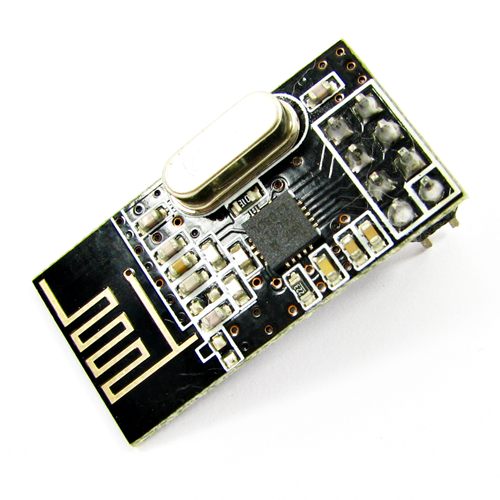
\includegraphics[width=0.5\linewidth]{../../Imagens/nordicc.png}
    \caption{Módulo de Rádio Frequência baseado no \textit{transceiver} da Nordic nRF24L01+}
    \label{Nordic}
  \end{figure}
Módulo de rádio frequência, vide  Fig. \ref{Nordic} obtida de \citeonline{nrf_image}, de baixo custo e consumo cuja faixa de operação situa-se na 
banda S das ondas UHF ( \textit{Ultra 
High Frequency} ), com uma porção dentro da banda ISM \footnote{maiores informações no apêndice}.
Algumas informações técnicas \cite{nRF} de interesse estão listadas abaixo: 
\begin{itemize}
 \item Tensão de alimentação: 1,9V - 3,6V
 \item Antena em circuito impresso do tipo MIFA(\textit{Meandered Inverted-F Antenna}) \cite{MIFA}
 \item Frequência de operação: 2,4GHz - 2,525GHz
 \item Modulação digital do tipo GFSK 
 \item Apresenta até 126 canais de comunicação \footnote{Válido apenas para as taxas de 250kbps e 1 Mbps; a 2Mbps este valor cai à metade, i.e. 63 
canais.}
 \item Taxas de bits: 250kbps, 1Mbps ou 2Mbps
 \item Potências de saída de transmissão: 0dBm, -6dBm, -12dBm e -18dBm
 \item Interface com o microcontrolador por SPI à taxa de até 10Mbps
 \item Pinos de entrada tolerantes a até 5V
 \item 
Pacotes recebidos verificados automaticamente, certificando-se da validade do endereço apontado e legitimando a integridade 
do pacote via CRC(\textit{Cyclic Redundancy Check}) \footnote{Vide apêndice para uma breve explanação sobre CRC}, antes de 
serem movidos às filas de dados recebidos (\textit{RX FIFO})
 \item Receptor envia ao transmissor um pacote de confirmação de recepção dos dados pelo mesmo canal (\textit{acknowledgment packet}).
\end{itemize}

\section{Arduino}
Trata-se de uma plataforma de prototipação eletrônica aberta, i.e. \textit{open-source hardware}, baseada no microcontrolador de 8 bits da Atmel 
ATMega328 \cite{ATMega}, programável via serial (ICSP) através de um microcomputador, por exemplo, por meio do ambiente de desenvolvimento 
\textit{Arduino Software IDE}, \textit{open-source software} e encontra-se no GitHub \cite{ArduSoft}.
Para programar este dispositivo, foi utilizado um módulo baseado na ponte USB-Serial PL-2303, cuja descrição detalhada pode ser encontrada em 
\citeonline{PL2303}.

Algumas informações técnicas \cite{ArduInfo} de interesse estão listadas abaixo: 
\begin{itemize}
 \item Dimensões: 17,78mm x 33mm
 \item Tensão de alimentação recomendável: 5V - 12V
 \item Memória 
 \begin{itemize}
  \item Flash: 32kB 
  \item SRAM: 2kB
  \item EEPROM: 1kB
 \end{itemize}

 \item 20 portas digitais de entrada/saída, das quais 6 podem ser usadas como saídas PWM
 \item 6 portas de entrada analógicas
 \item \textit{clock} de 16MHz
\end{itemize}


\section{Bateria} % TODO
Baterias do tipo LiPo são uma das mais indicadas para veículos elétricos e híbridos, tanto quanto para equipamentos eletrônicos portáteis; no 
entanto, alguns cuidados precisam ser tomados ao manipulá-la por serem sensíveis a sobrecarga ou descarga abrupta.
Logo, por questões de segurança e eficiência é necessário haver um sistema eletrônico para gerenciar a recarga deste dispositivo, o qual monitora a 
tensão de cada uma das células assim como a temperatura em pontos específicos \cite{battery}.
Neste trabalho foi utilizado o carregador IMAX B6-AC para fazer este serviço.
\subsection{\textit{C rate}}
É um parâmetro que descreve a corrente de descarga da bateria em relação à sua capacidade nominal \cite{bateria}.
Vide a Eq. \ref{C rate} para um exemplo ilustrativo baseado na bateria utilizada neste projeto.

\begin{equation}
 \label{C rate}
 30 C = \frac{ I_{descarga} }{ 2.800 mAh} \Rightarrow I_{descarga} \approx 10.7A
\end{equation}
